\subsection{Fazit}

Nach dem Aufgaben und der Wissensvermittlung unseres Workshops fassten wir nochmal alles zum Thema '"Emotion Tracking'" und '"Affective Computing'" zusammen. Wir erläuterten hierbei nochmal die Möglichkeiten Daten eines Nutzers zu erfassen, um den personenbezogenen Kontext zu verstehen. Die gesammelten Inforamtionen können über verschiedene Methoden klassifiziert werden.

\begin{figure}[!ht]
	\centering
	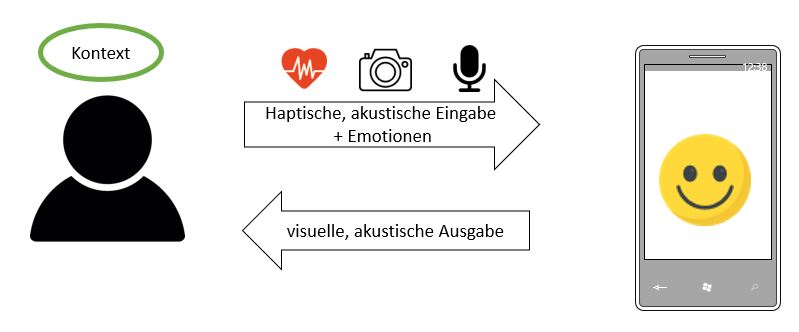
\includegraphics[width=0.9\linewidth]{Pictures/Fazit_Grafik}
	\caption[Verbesserung der MMI durch Emotion Tracking]{Verbesserung der \ac{HMI} durch Emotion Tracking}
	\label{fig:fazitgrafik}
\end{figure}

Das System kann eine Antwort geben, welche auf die Eingabe unter Berücksichtigung der Emotionen reagiert. Außerdem war es uns wichtig zu erwähnen, dass Emotion-Tracking nicht nur auf den Bereich Smartphones und weiteren mobilen Geräten anwenden lässt, sondern jeden Kommunikation zwischen Mensch und Maschine hiermit verbessert werden kann. 
